\chapter{Ciclo 2: Indexação com DTW}
\label{chap:dtw}

TODO: explicar a ideia do DTW vinda a partir dos resultados do primeiro ciclo

Uma forma de visualizar como os dados podem ser estruturados é transformando as sessões de uma música em uma espécie de máquina de estados. Por exemplo, uma máquina de estados da música \textit{Message In A Bottle}, para a trilha da guitarra, é ilustrada na \figref{fig:miab_state_machine}. No entanto, é notável que alguns estados podem transitar para mais de um estado. Por exemplo, a Introdução pode transitar entre si mesma em um \textit{loop} ou para o \textit{Bridge 1}. Tal característica quebra a Regra 3, pois, caso a sessão identificada fosse a introdução, não seria possível saber qual seria a próxima sessão e duas previsões seriam entregues.

\begin{figure}[htbp]
    \centering
    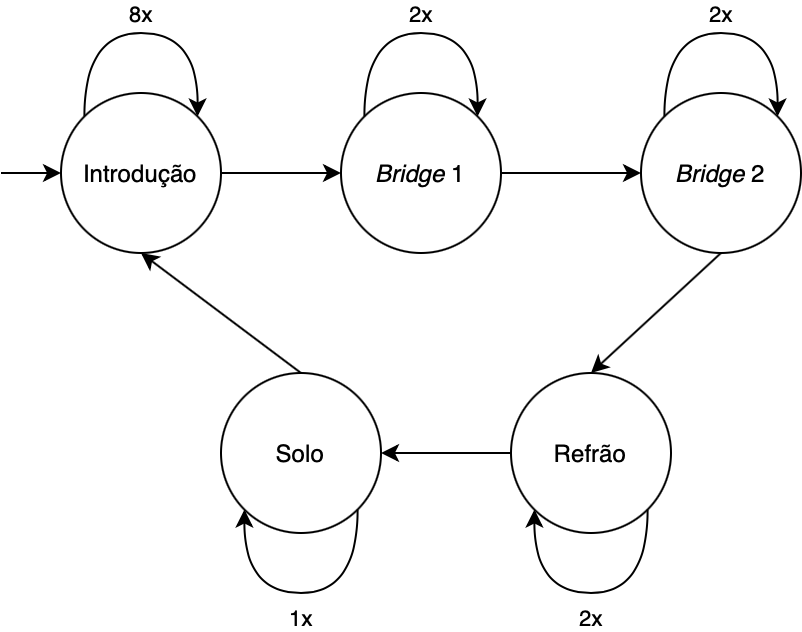
\includegraphics[width=0.75\textwidth]{images/MIAB state machine.png}
    \caption{Máquina de estados para a trilha da guitarra elétrica da música \textit{Message In A Bottle} (\textit{The Police}, 1979).}
    \label{fig:miab_state_machine}
\end{figure}

Para lidar com isso, podemos reorganizar tal máquina de estados apresentando sessões de transição entre os estados. Dessa forma, quando uma transição fosse identificada, apenas uma previsão seria gerada, como ilustrado na \figref{fig:miab_adapted_state_machine}. Note, entretanto, que nenhum dos estados "aponta" para um estado de transição. Isso significa que nenhuma das previsões conterá um desses estados, efetivamente perdendo essa informação de transição.

É importante, portanto, que cada estado represente um arquivo de música com curta duração. Dessa forma, mais estados poderão ser previstos e, portanto, mais correta serão as previsões.

\begin{figure}[htbp]
    \centering
    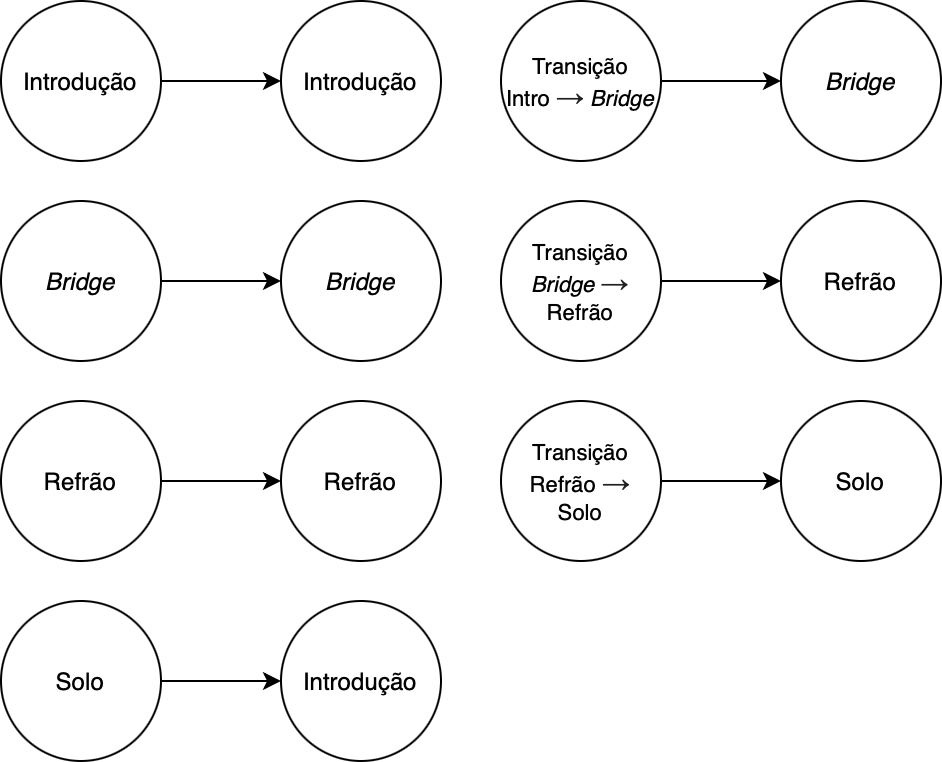
\includegraphics[width=0.4\textwidth]{images/MIAB adapted state machine.png}
    \caption{Máquina de estados adaptada para a trilha da guitarra elétrica da música \textit{Message In A Bottle} (\textit{The Police}, 1979).}
    \label{fig:miab_adapted_state_machine}
\end{figure}


Neste trabalho, realizamos a primeira técnica manualmente, ouvindo as músicas recolhidas na \secref{sec:data_gathering}, identificando as janelas de áudio diferentes entre si e indexando as janelas que vieram após cada uma. 